\section{助教(Teaching Assistant)怎么做}

\subsection{我是否需要做TA?}
\begin{itemize}
    \item 如果你是全额奖学金的博士生(免学费+有津贴),那根据学校发给你的的Financial offer,你每学期都有TA的义务(换句话说,奖学金是TA工作量换来的,拿了钱必须做事)。做了TA过后,不会另外结算工资。2020年及之后入学的全奖博士,三年需要做满900小时助教方可毕业。2023年及之后入学的全奖博士,每学年需要做300-500小时TA或RA方可毕业。
    \item 如果你是2020年及之后入学的半奖博士生(仅免学费)或者自费生,则没有做TA的义务。做TA过后,学校会按照工时给你发工资,而且TA的经历写到你简历上,(视你未来的职业规划)可能有一些作用。
\end{itemize}

全奖每学年强制300小时TA,按一年40个教学周计算,每周都有7.5小时的duty,相当于每周费掉一天。肯定有同学要问,真的会这么严格吗?从具体执行的情况来看,不同学院之间有很大区别。有的学院甚至专门为此建立了一个数字化系统来统计你的工时,然后必须作满;有的学院就比较佛。因此具体执行情况,请问你同专业的学长学姐。

\begin{flushright}
    (2022年10月21日 by Kai Wu)

    (major update: 2022年12月30日 by Yue Zhou: 根据最新官方handbook修正TA时间)

    (update: 2024年1月15日 by Kai Wu:根据最新官方handbook修正TA时间)
\end{flushright}

\subsection{如何成为一名TA}

每学期的第一周前后,学院会招募TA,一般由学院的秘书(School Academic Administrator)联系大家。
\begin{itemize}
    \item 半奖及自费博士比较自由,可自行与任课老师联系
    \item 全奖博士分两种情况:a.自行与任课教师联系 b.学院直接发邮件分配
\end{itemize}

如果你很想参加,或者想早点占某个科目、某为老师的坑,可以尽早联系秘书以及对应的科任老师。

\begin{flushright}
    (2022年12月30日 by Yue Zhou)
\end{flushright}

\subsection{TA的工作种类,以及分别怎么做}

助教的工作包括不局限于
\begin{enumerate}
    \item 批改作业及试卷
    \item 给本硕学生上tutorial(商科居多)、上lab
    \item 核算登记课程分数
    \item 做一些辅助性的工作(如设置Learning Mall等)
    \item 期中、期末监考
\end{enumerate}

研究生院会组织TA培训,以\textit{Teaching Assistant (TA) Training Programme}为题的邮件通知,也可以直接在你的Learning Mall上找到。每学期都有。如果一次都没去过,最好至少去听一次。下面是比较核心的、学校培训讲不太明白的内容:

\subsubsection{批作业}
如果是传统的改线下的纸质作业,一般问老师怎么做就行。如果是通过Learning Mall(以下简称LMO)提交的电子版作业,下面是教程:
\begin{enumerate}
    \item 登录LMO,找到你做助教的课程。如果翻遍了都找不到,需要发邮件给你们学院的秘书或者任课老师给你权限。
    \begin{figure}[H]
        \centering
        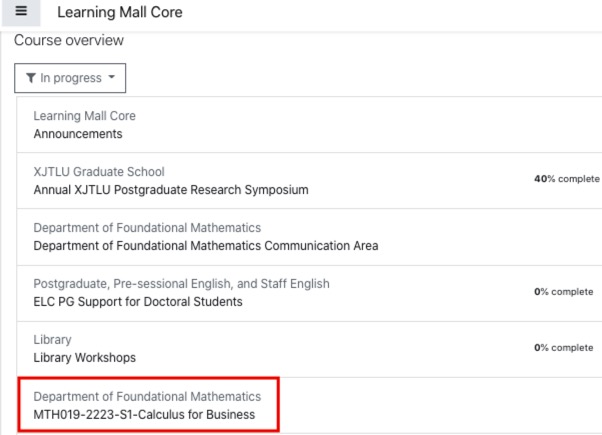
\includegraphics[width=0.4\columnwidth]{author-folder/Kai.Wu/LMO_course.jpg}
    \end{figure}

    \item 
    \begin{minipage}{0.3\textwidth}
        点进课程,往下拉找到提交作业的地方,或者直接用Ctrl+F(Mac:Command+F)搜索 submission
    \end{minipage}
    \begin{minipage}{0.63\textwidth}
        \begin{figure}[H]
            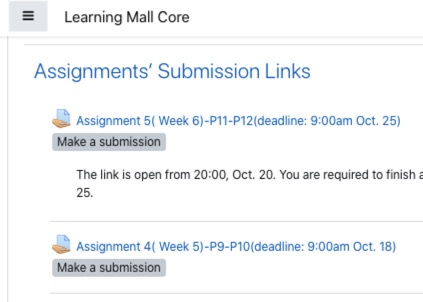
\includegraphics[width=0.95\columnwidth, right]{author-folder/Kai.Wu/LMO_submission_links.jpg}
        \end{figure}
    \end{minipage}

    \item 超大的必修课会有很多个班,先选择你被分配到改作业的班级(Seperate group)。接下来,如果你要马上开始在网页上在线批改,点击Grade。如果想看看,或者想离线批改(比如下载到iPad上),点击view all submission。
        \begin{figure}[H]
            \centering
            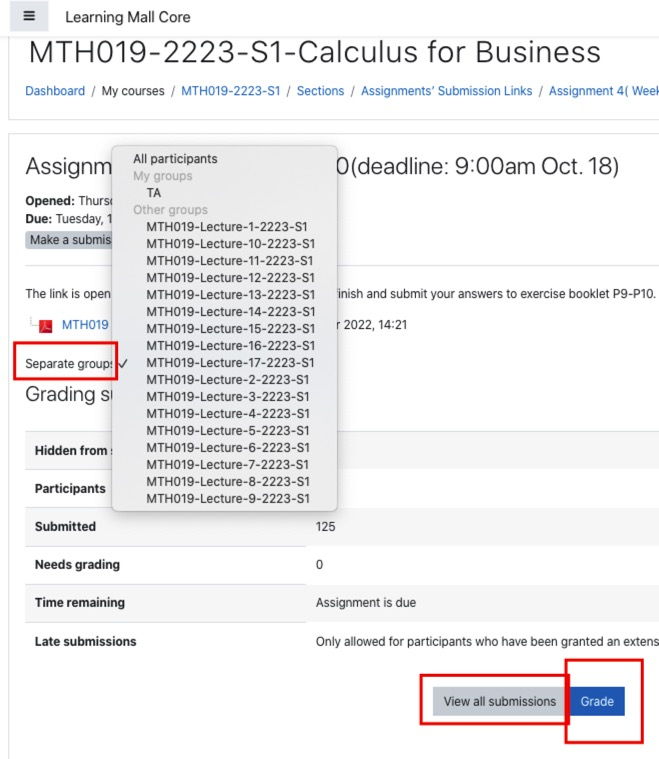
\includegraphics[width=0.5\columnwidth]{author-folder/Kai.Wu/LMO_inside_submission.jpg}
        \end{figure}
    \item 我对在线批改系统深恶痛绝,很卡,而且在线的PDF标记工具贼难用,改作业效率很低。除非老师做了打分表格(我导师给我展示过一次,在线批改的时候右边可以直接选择每个小题的分数,以及错误原因,这样就很高效,但我改过作业的module一个都没有做过这个),否则在线就很鸡肋。因此下面我只介绍我摸索出来的相对高效的离线批改方法。点进view all submission过后,在上面的grade action里,分别选择[下载成绩表]和[下载全部提交文件]
        \begin{figure}[H]
            \centering
            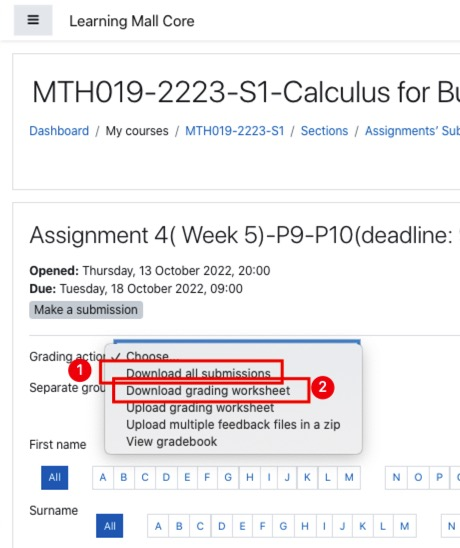
\includegraphics[width=0.5\columnwidth]{author-folder/Kai.Wu/LMO_download.jpg}
        \end{figure}
    \item 然后你就会获得一个csv文件和一个超级大zip。解压zip会看到所有学生提交的作业都以姓名+学号+一堆字命名好了。接下来你就可以把这堆文件在你电脑上、或者传到平板上本地批改。如果你的科任老师不要求把批改过的作业作为feedback file发回给学生(得问老师),你甚至可以全部打印出来改。改完过后,把成绩登到成绩表里。csv可以用Excel打开,你可以另存为xlsx格式。表格最后一列是Feedback comments,可以在里面写对学生要说的话,比如,文件格式不对、下次请拍清晰一点,之类的
        \begin{figure}[H]
            \centering
            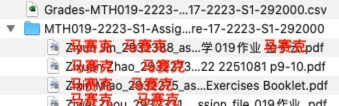
\includegraphics[width=0.5\columnwidth]{author-folder/Kai.Wu/LMO_Downloaded.jpg}
        \end{figure}
    \item 按照老师的要求改完作业过后,可以很方便的把成绩表和批改过的文件(如果老师要求)传回LMO。还是在刚才view all submission之后的页面,点击upload grading worksheet,把成绩表传上去。
        \begin{figure}[H]
            \centering
            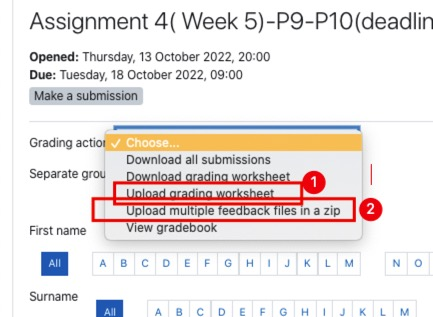
\includegraphics[width=0.5\columnwidth]{author-folder/Kai.Wu/LMO_upload.jpg}
        \end{figure}
    \item 要注意,如果你中间用Excel把它存成了xlsx,上传前需要另存为UTF-8的csv格式再上传。勾选下面allow那一句,允许表格内容覆盖已经在网页改过的内容。点击下面upload过后,你会看到很长一串网页,每个学生的成绩(和你输入的feedback comments)就传上去了。
        \begin{figure}[H]
            \centering
            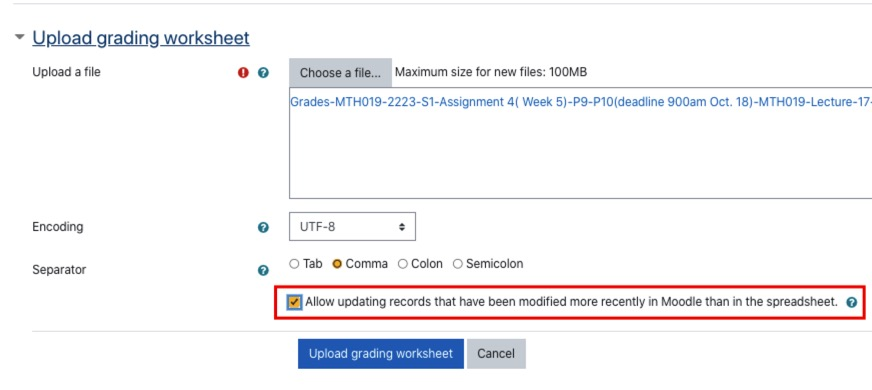
\includegraphics[width=0.8\columnwidth]{author-folder/Kai.Wu/LMO_upload_sheet.jpg}
        \end{figure}
    \item 回到刚才的页面,点upload multiple feedback files in a zip,上传批改过的作业文件。把作业文件打包成zip上传,但由于LMO限制上传大小不能超过100M,如果总大小超过了就要手动打包成多个小于100M的zip(神烦,为什么下载就可以超过100M)。会用Python的,可以用我随便写的这个Python脚本 \href{https://github.com/kaiwu-astro/xp_pgrs_unofficial_guide/tree/main/fileshare/zip_in_100M.py}{GitHub链接} 或 \href{https://gitee.com/kaiwu-astro/xp_pgrs_unofficial_guide/tree/main/fileshare}{不能上GitHub的用这个链接},来自动按最大100M打包成多个文件(如果不会Python当然还是手动打包比较快)。上传完过后就完事了。
    \item 最后要发邮件给老师,说明(1)发现的共性问题,比如某道题错得很多,某道题不会的很多,某道题有的学生错理解成了什么,之类的,(2)个别问题,例如某学生交错了文件,某学生疑似抄袭标准答案(这种一般是高年级学生给他的),某学生和某学生作业雷同,(3)以及其他任何想和老师沟通的问题。大学数学系有下面这种专门的反馈表,填到表里。如果没有反馈表的,给老师发邮件说下也可以。(一般都不用太详细,不要学我,很费时间,除非你热爱这项事业)
        \begin{figure}[H]
            \centering
            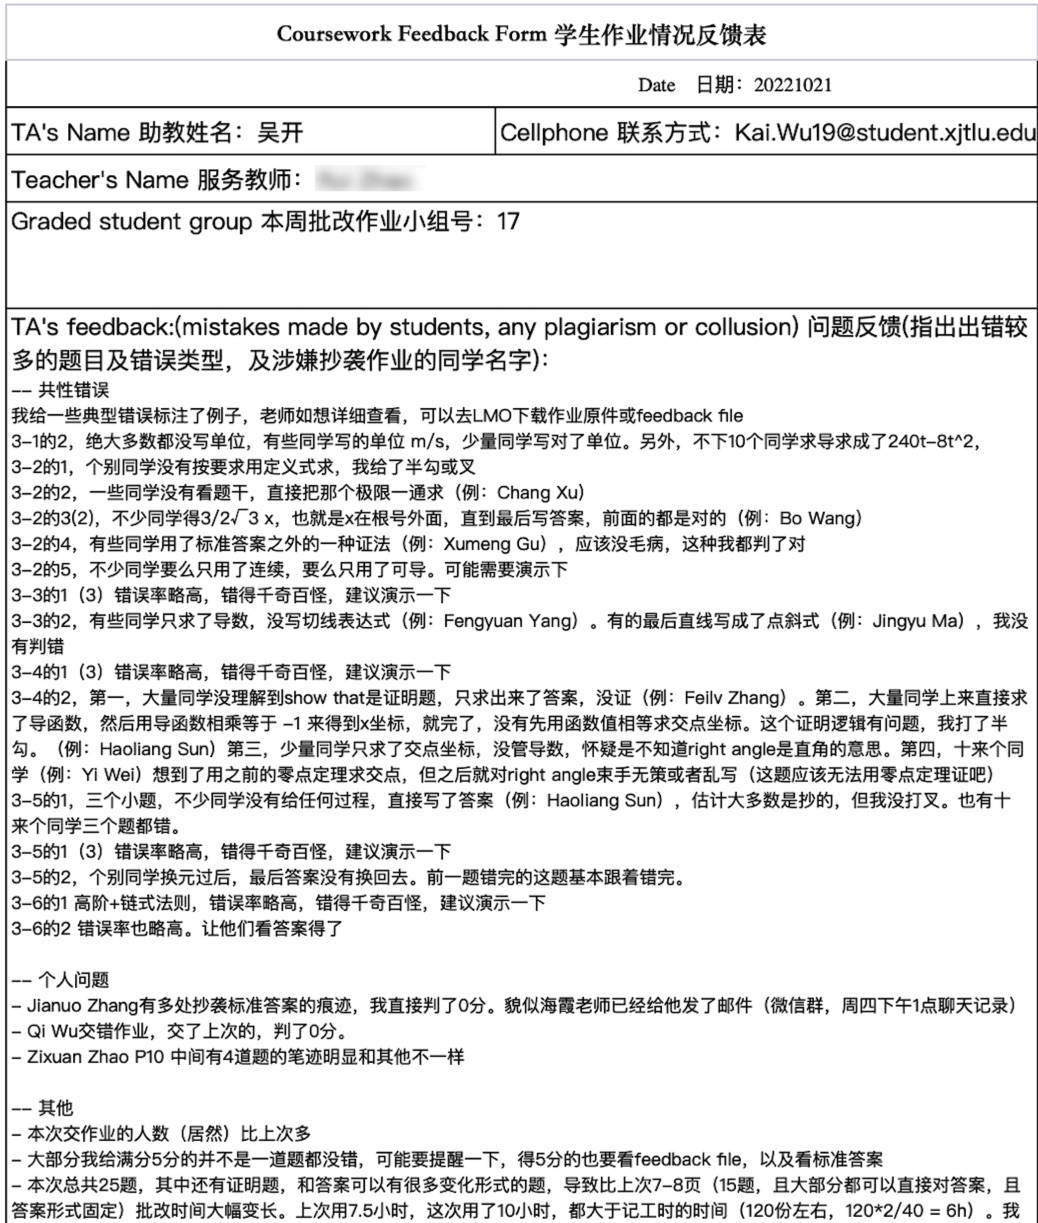
\includegraphics[width=0.5\columnwidth]{author-folder/Kai.Wu/LMO_feedback_to_teacher.jpg}
        \end{figure}
\end{enumerate}


\emptyline
【分享一下我的批作业经验】
\begin{enumerate}
    \item 我的工具组合是iPad + Apple pencil + PDF Expert app,比在电脑上在线、离线改都快得多。另外如果购买磁吸类纸膜(约20元)+ pencil替换笔头(约10元),会大幅提高书写体验
        \begin{figure}[H]
            \centering
            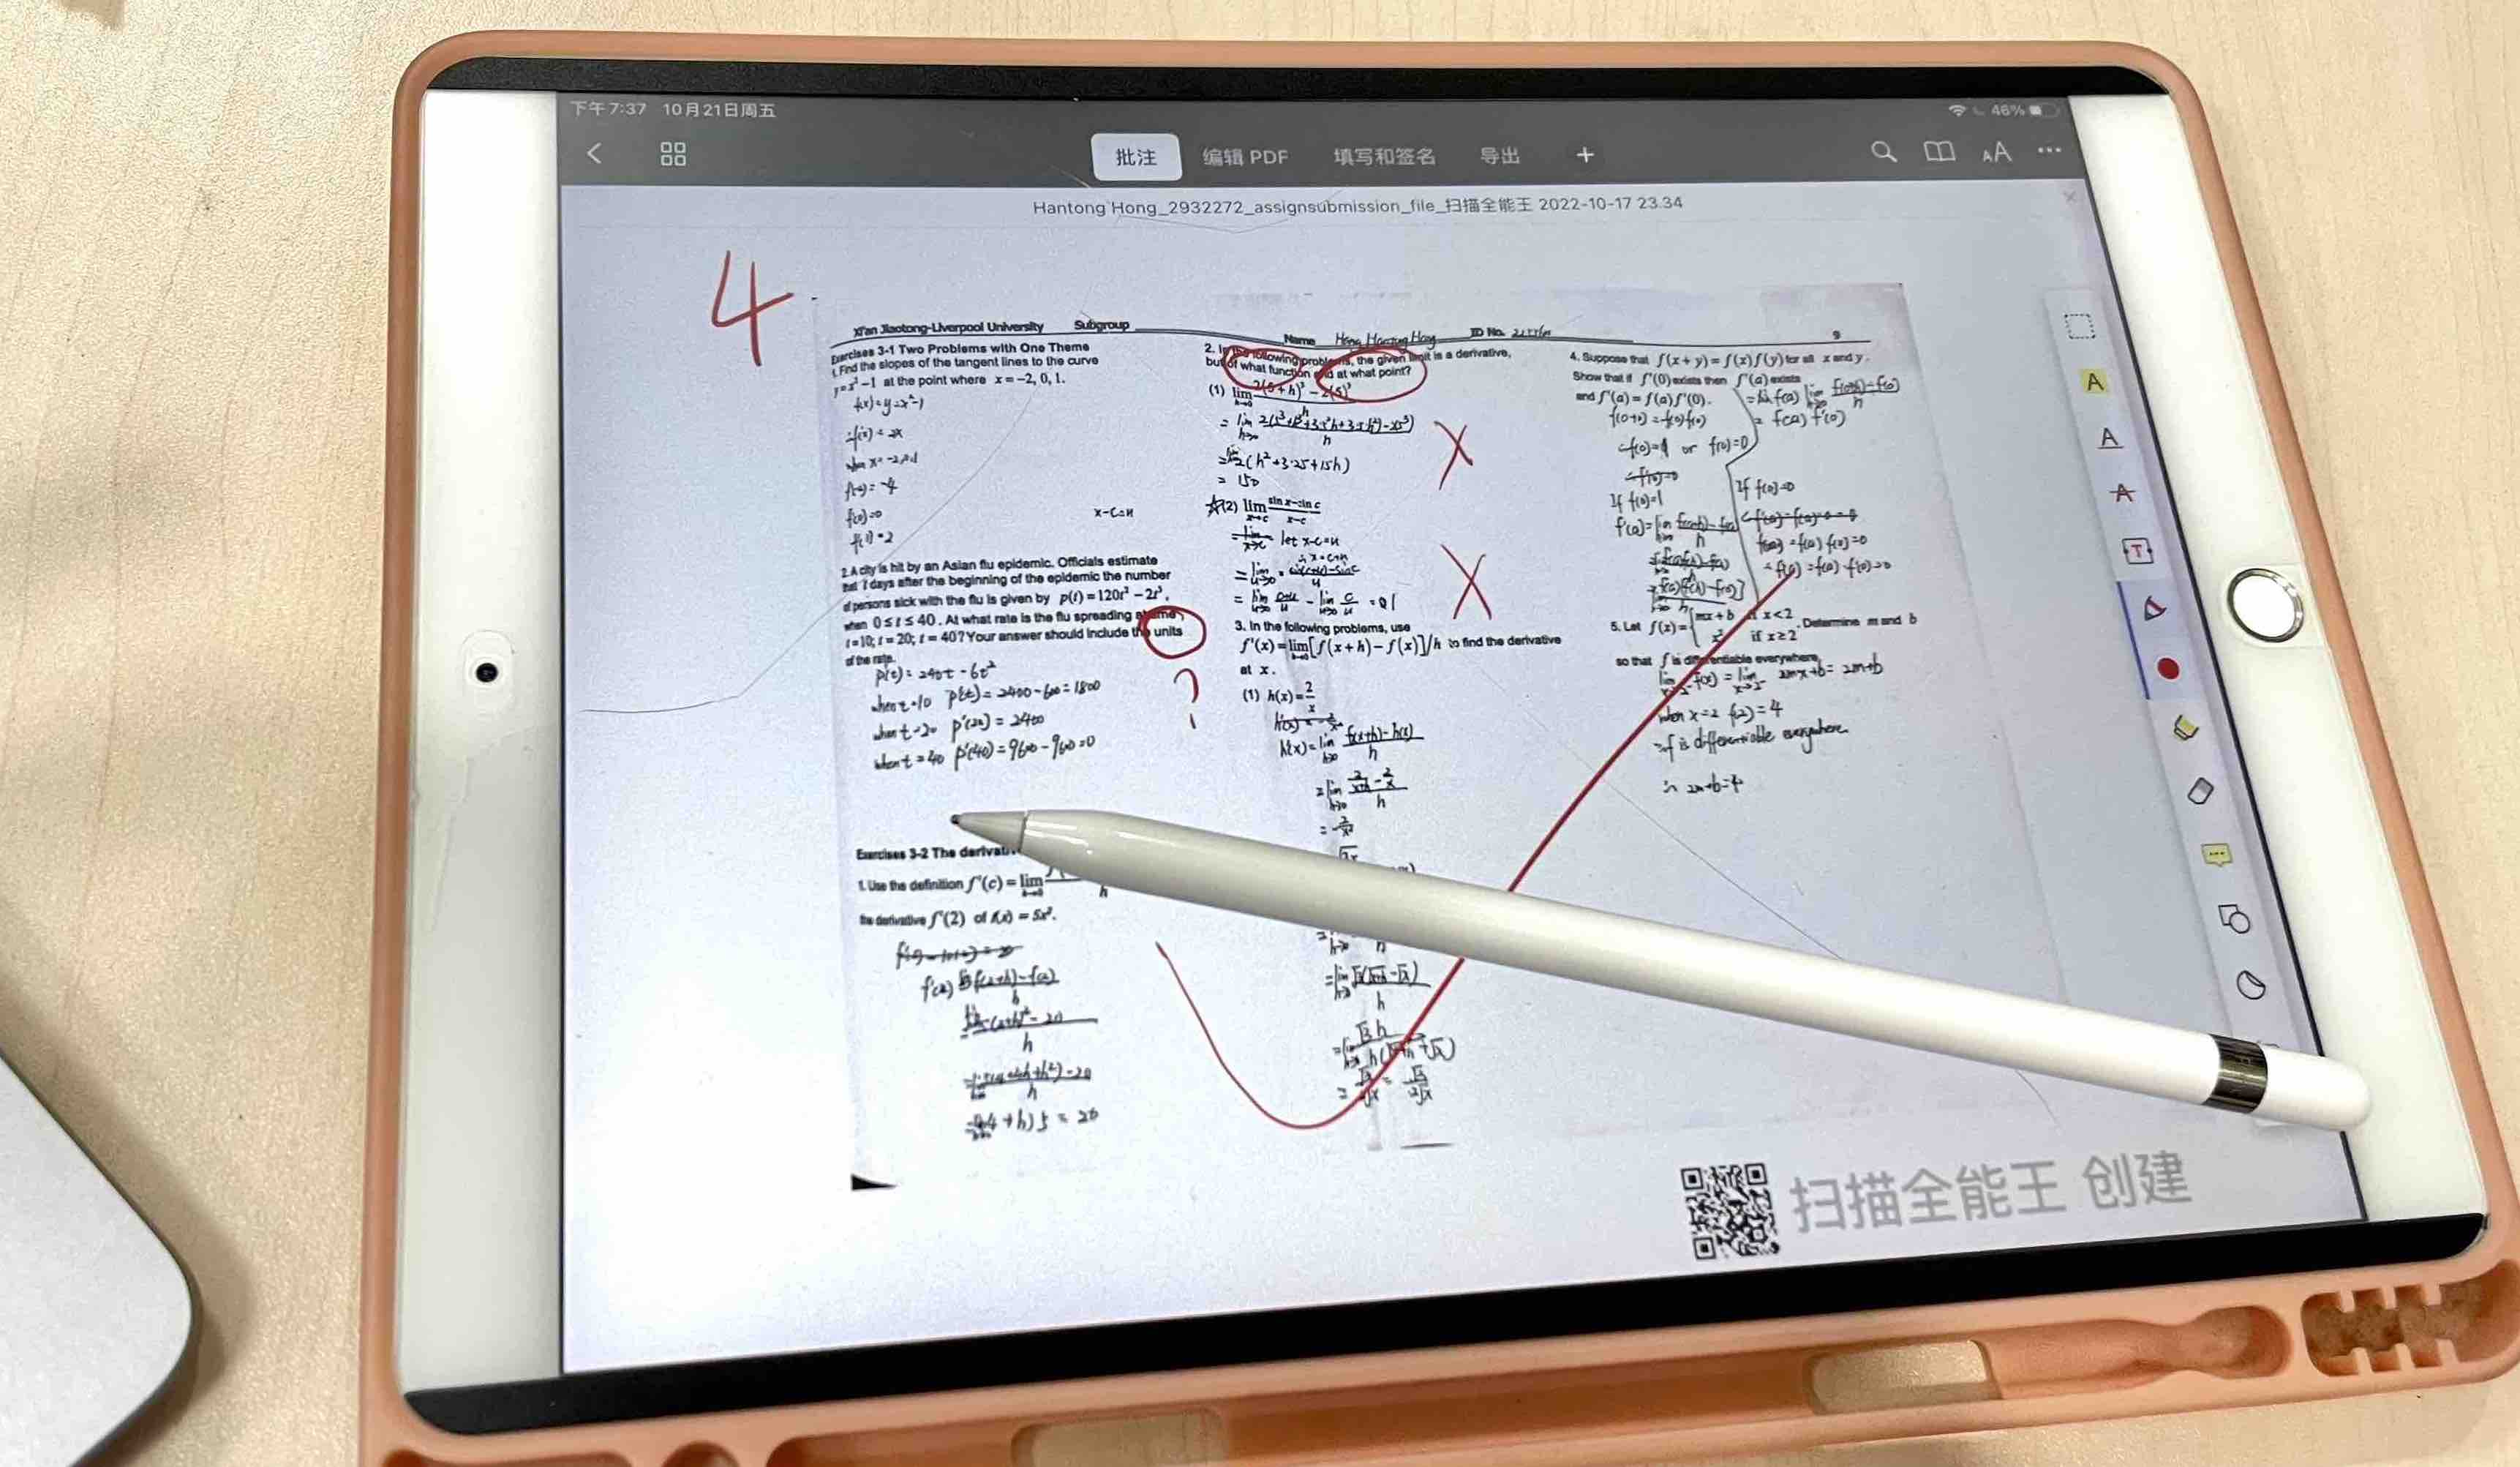
\includegraphics[width=0.5\columnwidth]{author-folder/Kai.Wu/marking_tools.jpg}
        \end{figure}
    \item 流水线提高效率:题多的时候,不要全部改完一个学生的作业再改下一份,这样尤其慢。尝试一下把作业分成几部分,先把所有作业的part 1(比如,前面三道题)改完,然后回过头来,改所有人的部分part 2(比如4-6题)。可能打开关闭文件会费一些时间,但这样能记住几个题的答案和评分点,改起来很快。切忌改每个作业都去看几眼答案。
    \item 同理,不要改完一个就登一个成绩。我的习惯是,把总成绩写一个巨大数字在左上角。全部改完过后,传电脑上,用最大号的缩略图(Mac:显示为图标,狂按command+等号;win:显示为超大图标),直接不打开文件就能看到左上角的分数。Excel里按姓名排序,文件夹里用名称排序,统起成绩来特别快。
        \begin{figure}[H]
            \centering
            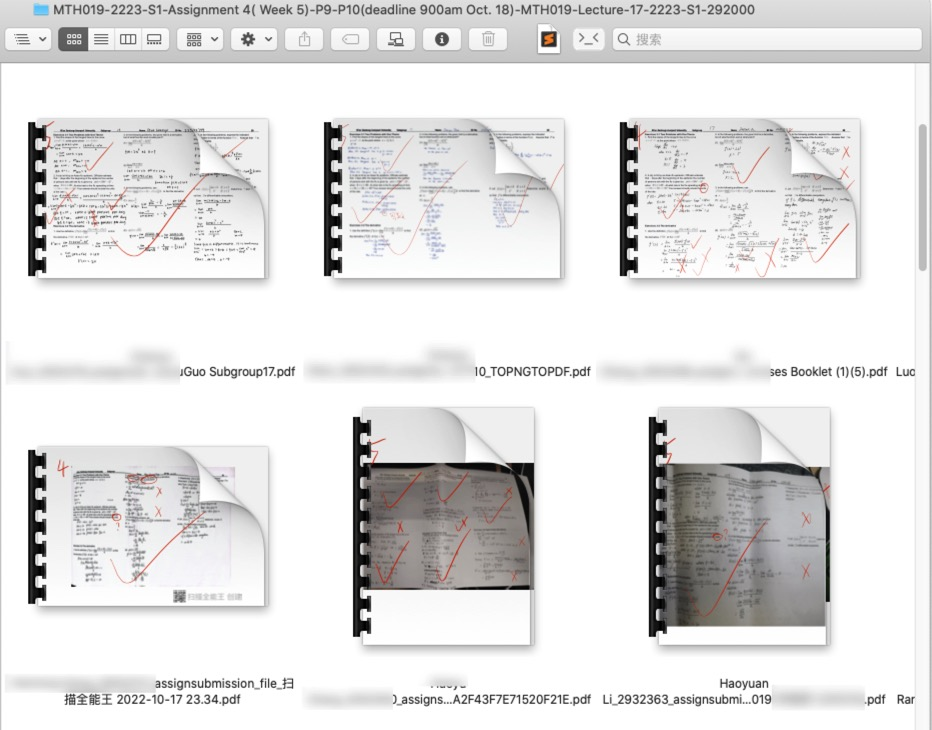
\includegraphics[width=0.7\columnwidth]{author-folder/Kai.Wu/tongchengji.jpg}
        \end{figure}
    \item 学生提交的文件可能有很多大病。比如,提交的不是pdf而是word甚至ppt、提交的pdf里面图片顺序是乱的、图片方向是错的、有标准的习题册不用而是自己拿个本写导致不好对答案。TA有权要求学生交作业的格式,可以对这些学生在feedback comments里面警告,并且提醒科任老师一定要在课上提醒学生,否则真的非常影响批阅效率。学生警告了仍然乱交格式时,可以按你的标准扣格式分。比如我的标准是:初犯警告,再犯扣20\%,三次扣50\%,四次扣完。
    \item 有时候文件巨大或者文件中有太多手写字迹,会导致pdf打开加载非常慢(一分钟甚至几分钟),而且容易崩溃。前者可以要求学生自行压缩PDF,后者实在是没办法。我写了一个Python程序\href{https://github.com/kaiwu-astro/xp_pgrs_unofficial_guide/tree/main/fileshare/pdf_to_png_to_pdf.py}{[GitHub链接]}应对这种情况,会在下载完所有作业过后把所有PDF转成图片再转回PDF,这样打开就不成问题了,文件大小也都能压缩到5M以内。需要的自取,但使用有点麻烦,不过我实在找不到其他更科学的方法了。
    \item (悄悄说)拿不准给多少分合适的时候,就给多一点。给少了,学生会找你argue,很浪费时间。给多一点,相当于节约自己的时间。
    \item 往表格登成绩的时候,难免犯错,登错或者登串成绩。初次或者前几次登成绩尤其容易出问题,可以考虑全部double check一遍。另外,如果你把成绩写在了PDF左上角,能一定程度解决这个问题,也就是如果成绩登错了,学生发现LMO成绩和PDF上的不一样,能马上联系你。
    \item 改完作业后,学生有可能会通过LMO给你发消息,或者给你发邮件。尽量不要直接回复学生,毕竟回复错了的话老师背锅。任何学生发给你的消息,请转给老师,让老师回复他。除非老师同意你直接回复。
\end{enumerate}

\begin{flushright}
    (2022年10月21日 by Kai Wu)
\end{flushright}

\subsubsection{批改试卷}
Quiz,期中,期末考试,助教有可能要参加评卷。所以期末放假跑路之前跟老师问清楚,以免要改期末卷但是不知道。如果确实有事要提前跑路,和老师商量。

\subsubsection{带Lab(实验课)}
\begin{newminipage}[0.55]
    像大学物理实验这种课,会让TA带实验课。物理实验的讲课流程一般是:先在实验室的白板给学生讲一下实验原理、数据如何记录和处理、注意事项,然后要亲手演示如何做实验。课后,要批改实验报告。

    我感觉,实验课非常有挑战性,因为确实就是实实在在的在大学里讲课。你需要自己花时间备课、准备讲稿、理清思路、准备学生可能问的各种问题;讲课前科任老师会对TA在实验室培训,你自己得先吃透如何做实验。还有突发事件如何处理,比如学生弄坏器材(及时问老师)。因为实验课就那么几节,总的工作时长加上批实验报告也比大部分其他课的批作业时长要少,但是非常锻炼人。可以挑战自己,如果不想干也一定要尽早跟老师、学院秘书提出换到其他课程。
    \begin{flushright}
        (2022年10月22日 by Kai Wu)
    \end{flushright}
\end{newminipage}
%
\begin{newminipage}[0.45]
    \begin{figure}[H]
        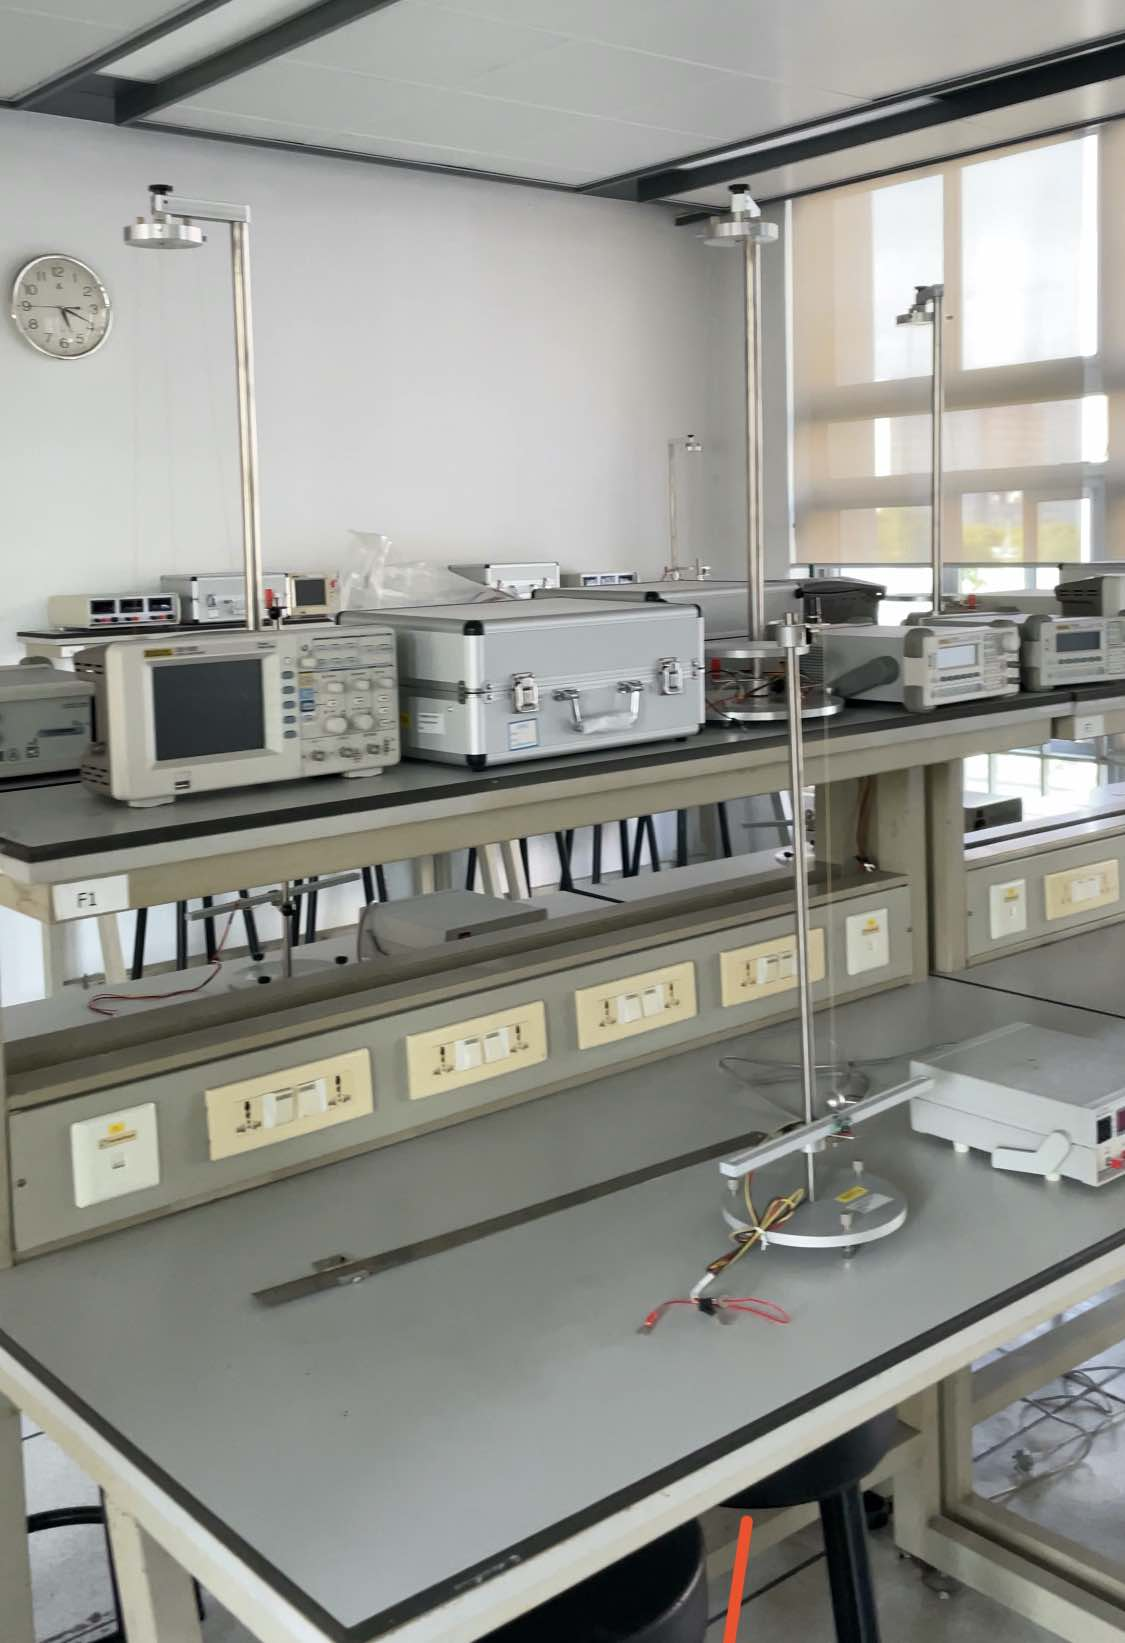
\includegraphics[width=0.95\columnwidth, right]{author-folder/Kai.Wu/lab.jpg}
    \end{figure}
\end{newminipage}



\subsubsection{如何做好讲Tutorial(习题课)}

\begin{enumerate}
    \item 课前做好充分准备工作,当你站上讲台那一刻,你就是一名教师了,要为自己说的所有的话负责,也要对学生负责。课前将课程所需要的材料拷到U盘中,进入教室后打开电脑登录自己的账号即可使用电脑。同时你也需要使用账号登录LM, AMS等乱起八糟的系统。由于学校电脑较卡顿,建议大家提前十分钟到达教室。此外,也需要提前十分钟下课,否则会被后面上课的老师和学生投诉你拖堂。
    \item 课后耐心回复学生的邮件与提问。此处给大家一个忠告,不要加轻易加学生微信,让他们有事有问题跟你邮件联系。否则你会变成一个7*24客服。邮件作为学校官方交流方式,很好的保护了教师和助教的私人空间和权益。曾经有学生投诉,就因为助教没有回复学生的微信。
    \item 有问题及时跟module leader沟通,遇到棘手的问题,不要自作主张,需要与module leader商量。学生给的反馈,也可以与co-teacher沟通,以提升学生的学习体验。学生体验感好了Module Questionnaire(MQ)分数自然就上去了。MQ的分数即学生评教分数,如果分数好看,求职的时候,是可以放到简历里的。
\end{enumerate}

\begin{flushright}
    (2022年12月30日 by Yue Zhou)
\end{flushright}

\subsection{TA工资是多少,怎么结}
2022年TA工资是60元/小时,每月一结,次月月底发钱。例如,2月底发1月工作的工资。

\emptyline{}
另外,期中、期末考试的监考也是TA的一种,会计入奖学金学生的TA工时,对自费同学,监考的工资单价一般也高得多。监考见下一节。
